\documentclass[a4paper,UTF8]{article}
\usepackage{ctex}
\usepackage[margin=1.25in]{geometry}
\usepackage{color}
\usepackage{graphicx}
\usepackage{amssymb}
\usepackage{amsmath}
\usepackage{amsthm}
\usepackage{enumerate}
\usepackage{bm}
\usepackage{hyperref}
\usepackage{pgfplots}
\usepackage{epsfig}
\usepackage{color}
\usepackage{mdframed}
\usepackage{lipsum}
\usepackage{algorithm}  
\usepackage{algpseudocode}  
\newmdtheoremenv{thm-box}{myThm}
\newmdtheoremenv{prop-box}{Proposition}
\newmdtheoremenv{def-box}{定义}
\newmdtheoremenv{theorem}{定理}

\usepackage{listings}
\usepackage{xcolor}
\lstset{
	numbers=left, 
	numberstyle= \tiny, 
	keywordstyle= \color{ blue!70},
	commentstyle= \color{red!50!green!50!blue!50}, 
	frame=shadowbox, % 阴影效果
	rulesepcolor= \color{ red!20!green!20!blue!20} ,
	escapeinside=``, % 英文分号中可写入中文
	xleftmargin=2em,xrightmargin=2em, aboveskip=1em,
	framexleftmargin=2em
} 

\setlength{\evensidemargin}{.25in}
\setlength{\textwidth}{6in}
\setlength{\topmargin}{-0.5in}
\setlength{\topmargin}{-0.5in}
% \setlength{\textheight}{9.5in}
%%%%%%%%%%%%%%%%%%此处用于设置页眉页脚%%%%%%%%%%%%%%%%%%
\usepackage{fancyhdr}
\usepackage{lastpage}
\usepackage{layout}
\footskip = 10pt
\pagestyle{fancy}                    % 设置页眉
\lhead{2018年春季}
\chead{机器学习导论}
% \rhead{第\thepage/\pageref{LastPage}页}
\rhead{作业五}
\cfoot{\thepage}
\renewcommand{\headrulewidth}{1pt}  			%页眉线宽,设为0可以去页眉线
\setlength{\skip\footins}{0.5cm}    			%脚注与正文的距离
\renewcommand{\footrulewidth}{0pt}  			%页脚线宽,设为0可以去页脚线

\makeatletter 									%设置双线页眉
\def\headrule{{\if@fancyplain\let\headrulewidth\plainheadrulewidth\fi%
\hrule\@height 1.0pt \@width\headwidth\vskip1pt	%上面线为1pt粗
\hrule\@height 0.5pt\@width\headwidth  			%下面0.5pt粗
\vskip-2\headrulewidth\vskip-1pt}      			%两条线的距离1pt
 \vspace{6mm}}     								%双线与下面正文之间的垂直间距
\makeatother

%%%%%%%%%%%%%%%%%%%%%%%%%%%%%%%%%%%%%%%%%%%%%%
\numberwithin{equation}{section}
%\usepackage[thmmarks, amsmath, thref]{ntheorem}
\newtheorem{myThm}{myThm}
\newtheorem*{myDef}{Definition}
\newtheorem*{mySol}{Solution}
\newtheorem*{myProof}{Proof}
\newtheorem*{myRemark}{备注}
\newcommand{\indep}{\rotatebox[origin=c]{90}{$\models$}}
\newcommand*\diff{\mathop{}\!\mathrm{d}}

\usepackage{multirow}

%--

%--
\begin{document}
\title{机器学习导论\\
作业五}
\author{151220097,孙旭东,248381185@qq.com}
\maketitle
\section{[30pts] Conditional Independence in Bayesian Network}
\begin{enumerate}[(1)]
	\item \textbf{[5pts]} 请给出图中贝叶斯网结构的联合概率分布的分解表达式。
	
	\label{structure1}
	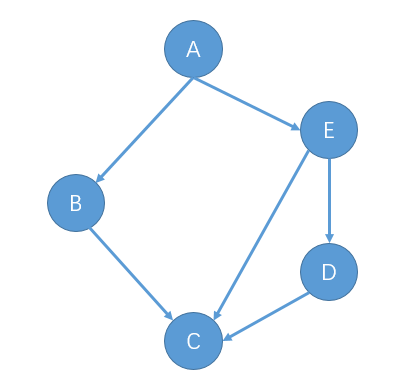
\includegraphics[width=7cm]{structure1.png}
	\item \textbf{[5pts]} 请给出下图中按照道德化方法可以找到的所有条件独立的组合(即哪些变量关于哪些变量或者变量集条件独立),独立也算做条件独立的一种特例。
	
	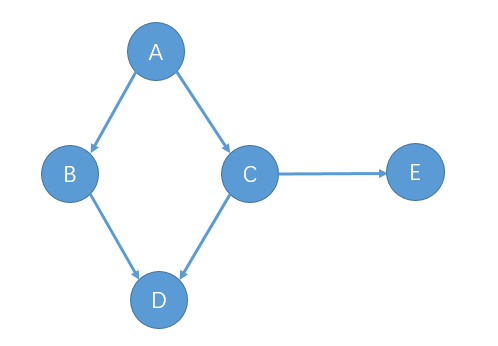
\includegraphics[width=9cm]{structure2.png}
	
	
	\item \textbf{[10pts]} 在这里,首先我们将给出关于“阻塞”的概念,然后我们根据“阻塞”的概念给出条件独立的充要条件。(大家也可以参考\href{http://www.andrew.cmu.edu/user/scheines/tutor/d-sep.html#formaldef}{这个网站})
	\begin{def-box}[阻塞]
		设$X,Y,Z$分别是一个有向无环图$G$里互没有交集的结点集,$Z$阻塞$X$中的一结点到Y中一结点的通路$P$(关于“通路”,在这里只要连通就算一条通路,对路中每条边的方向无任何要求),当且仅当满足以下条件之一:
		
		1. $P$中存在顺序结构$x\rightarrow z\rightarrow y$或同父结构$x\leftarrow z\rightarrow y$,结点$z$包含在集合$Z$中;
		
		2. $P$中存在V型结构$x\rightarrow z \leftarrow y$,结点$z$及其孩子结点不包含在集合Z中。
		
	\end{def-box}
	\begin{theorem}[条件独立]
		\label{theorem}
		设$X,Y,Z$分别是一个有向无环图$G$里互没有交集的结点集,如果集合$Z$阻塞$X$到$Y$的任何一条道路,则$X$和$Y$在给定$Z$时条件独立,即$X\indep Y|Z$。
	\end{theorem}
	请根据定理\ref{theorem},判断第一问中有哪些条件独立的组合(独立也算条件独立的一种特例)。
	
	\item \textbf{[10pts]} 由以上两问我们可知,道德化方法中的“除去集合$z$后,$x$和$y$分属两个连通分支”并不构成条件独立性的充要条件。如果对道德化方法稍加修改,在连接V型结构父结点前,我们只保留图中$X,Y,Z$及他们的非孩子结点,之后的步骤则相同。请问你认为用修改后的方法可以保证得到{\color{red}{全部的}}正确的条件独立集合吗?如果可以,请说明理由;如果不能,请给出反例。
	
\end{enumerate}
\begin{myProof}
	此处用于写证明(中英文均可)
	~\\
\begin{enumerate}[(1)]
\item 
\begin{equation}
\begin{aligned}
&P(A,B,C,D,E)\\ 
=& P(A)P(B|A)P(C|B,D,E)P(D|E)P(E|A)
\end{aligned}
\end{equation}
\item 
条件独立的组合:\\
\begin{equation}
\begin{aligned}
&E \perp A | C\\
&E \perp B | C\\
&E \perp D | C\\
&A \perp D | B, C\\
\end{aligned}
\end{equation}
还有一些冗余的条件独立组合,也属于合法的条件独立组合
\begin{equation}
\begin{aligned}
&E \perp A | C, B\\
&E \perp A | C, D\\
&E \perp A | C, B, D\\
&E \perp B | C, A\\
&E \perp B | C, D\\
&E \perp B | C, A, D\\
&E \perp D | C, A\\
&E \perp D | C, B\\
&E \perp D | C, A, B\\
&A \perp D | B, C, E
\end{aligned}
\end{equation}
\item 
条件独立的组合:\\
\begin{equation}
\begin{aligned}
&A \indep C | B,E\\
&A \indep C | B,E,D\\
&A \indep D | E\\
&A \indep D | B,E\\
&B \indep D | A\\
&B \indep D | E\\
&B \indep D | A,E\\
&B \indep E | A\\
&B \indep E | A,D
\end{aligned}
\end{equation}
\item 
不可以得到全部的正确的条件独立的组合,反例如下:
\begin{figure}[!ht]
	\centering
	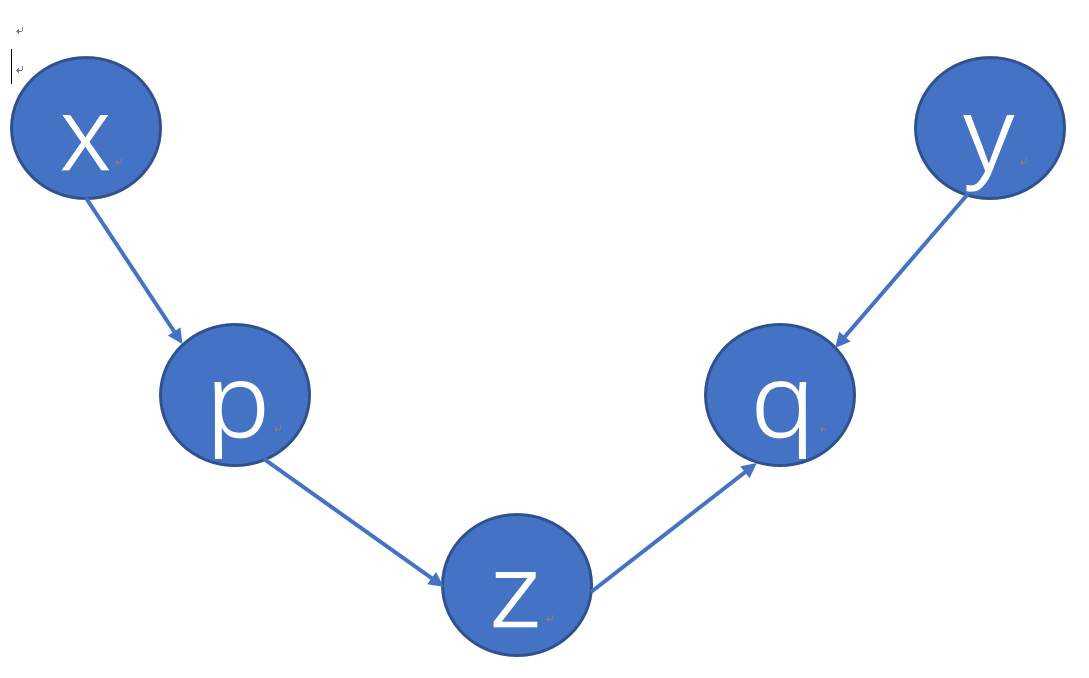
\includegraphics[scale=0.5]{bayes.png}
	\caption{反例}
	\label{fig:label2}
\end{figure}\\\\
按照充要条件,有:
\begin{equation}
x \indep y | z
\end{equation}
\\
但是根据题意,a作为x的子节点会被删除,那么x和y不再连通:\\
\begin{figure}[!ht]
	\centering
	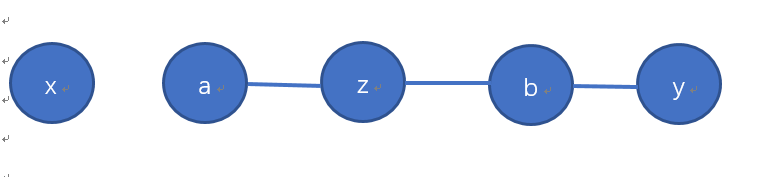
\includegraphics[scale=0.5]{bayes2.png}
	\caption{反例}
	\label{fig:label3}
\end{figure}\\
就有x和y直接独立,不能得到上述条件独立的组合。\\
\end{enumerate}
\end{myProof}
\newpage
\section{[20pts] Naive Bayes Classifier}
	
	通过对课本的学习,我们了解了采用“属性条件独立性假设”的朴素贝叶斯分类器。现在我们有如下表所示的一个数据集:
	\begin{table}[htp]
		\centering
		\caption{数据集}\label{tab:aStrangeTable}
	\begin{tabular}{c|ccccc}
		\hline 
	编号	& $x_1$ & $x_2$ & $x_3$ & $x_4$ & $y$ \\ 
		\hline 
	样本1	& 1 & 1 & 1 & 0 & 1 \\ 
		\hline 
	样本2	& 1 & 1 & 0 & 0 & 0 \\ 
		\hline 
	样本3	& 0 & 0 & 1 & 1 & 0 \\ 
		\hline 
	样本4	& 1 & 0 & 1 & 1 & 1 \\ 
		\hline 
	样本5	& 0 & 0 & 1 & 1 & 1 \\ 
		\hline 
	\end{tabular}
	\end{table} 
	
	\begin{enumerate}[ {(}1{)}]
		\item \textbf{[10pts]} 试计算:$\Pr\{ y=1 | \mathbf{x}=(1,1,0,1) \}$ 与 $\Pr\{ y=0 | \mathbf{x}=(1,1,0,1) \}$ 的值;
		\item \textbf{[10pts]} 使用“拉普拉斯修正”之后,再重新计算上一问中的值。
	\end{enumerate}
	
\begin{mySol}
	~\\
\begin{enumerate}[ {(}1{)}]
\item 
\begin{equation}
\Pr\{ y=1 | \mathbf{x}=(1,1,0,1) \} = \frac{\Pr\{\mathbf{x}=(1,1,0,1) | y=1  \} \Pr\{y=1\}}{\Pr\{\mathbf{x}=(1,1,0,1) \}}
\end{equation}
根据“属性条件独立性假设”的思想,有:
\begin{equation}
\begin{aligned}
&\Pr\{\mathbf{x}=(1,1,0,1) | y=1  \}\\ 
=& \Pr\{x_1 = 1 | y = 1\}\Pr\{x_2 = 1 | y = 1\}\Pr\{x_3 = 0 | y = 1\}\Pr\{x_4 = 1 | y = 1\}\\
=& \frac{2}{3}\times\frac{1}{3}\times\frac{0}{3}\times\frac{2}{3}\\
=& 0
\end{aligned}
\end{equation}
以及
\begin{equation}
\begin{aligned}
&\Pr\{\mathbf{x}=(1,1,0,1)\}\\ 
=& \Pr\{x_1 = 1\}\Pr\{x_2 = 1\}\Pr\{x_3 = 0\}\Pr\{x_4 = 1\}\\
=& \frac{3}{5}\times\frac{2}{5}\times\frac{1}{5}\times\frac{3}{5}\\
=& \frac{18}{625}
\end{aligned}
\end{equation}
所以可得:
\begin{equation}
\Pr\{ y=1 | \mathbf{x}=(1,1,0,1) \} = 0
\end{equation}
类似的
\begin{equation}
\Pr\{ y=0 | \mathbf{x}=(1,1,0,1) \} = \frac{\Pr\{\mathbf{x}=(1,1,0,1) | y=0  \} \Pr\{y=0\}}{\Pr\{\mathbf{x}=(1,1,0,1) \}}
\end{equation}
根据“属性条件独立性假设”的思想,有:
\begin{equation}
\begin{aligned}
&\Pr\{\mathbf{x}=(1,1,0,1) | y=0  \}\\ 
=& \Pr\{x_1 = 1 | y = 0\}\Pr\{x_2 = 1 | y = 0\}\Pr\{x_3 = 0 | y = 0\}\Pr\{x_4 = 1 | y = 0\}\\
=& \frac{1}{2}\times\frac{1}{2}\times\frac{1}{2}\times\frac{1}{2}\\
=& \frac{1}{16}
\end{aligned}
\end{equation}
以及
\begin{equation}
\Pr\{\mathbf{x}=(1,1,0,1)\} = \frac{18}{625}
\end{equation}
又因为
\begin{equation}
\Pr\{y=0\} = \frac{2}{5}
\end{equation}
综上可得
\begin{equation}
\begin{aligned}
&\Pr\{ y=0 | \mathbf{x}=(1,1,0,1) \}\\ 
=& \frac{\Pr\{\mathbf{x}=(1,1,0,1) | y=0  \} \Pr\{y=0\}}{\Pr\{\mathbf{x}=(1,1,0,1) \}}\\
=& \frac{\frac{1}{16}\times\frac{2}{5}}{\frac{18}{625}}\\ 
=& \frac{125}{144} 
\end{aligned}
\end{equation}

\item 
首先有:
\begin{equation}
\Pr\{\mathbf{x}=(1,1,0,1)\} = \frac{18}{625}
\end{equation}
根据上题,结合“拉普拉斯修正”,可得:
\begin{equation}
\begin{aligned}
&\Pr\{\mathbf{x}=(1,1,0,1) | y=1  \}\\ 
=& \Pr\{x_1 = 1 | y = 1\}\Pr\{x_2 = 1 | y = 1\}\Pr\{x_3 = 0 | y = 1\}\Pr\{x_4 = 1 | y = 1\}\\
=& \frac{3}{5}\times\frac{2}{5}\times\frac{1}{5}\times\frac{3}{5}\\
=& \frac{18}{625}
\end{aligned}
\end{equation}
还有:
\begin{equation}
\Pr\{y=1\} = \frac{4}{7}
\end{equation}
所以得到:
\begin{equation}
\Pr\{ y=1 | \mathbf{x}=(1,1,0,1) \} = \frac{4}{7}
\end{equation}
类似的,根据"拉普拉斯修正",可得:
\begin{equation}
\begin{aligned}
&\Pr\{\mathbf{x}=(1,1,0,1) | y=0  \}\\ 
=& \Pr\{x_1 = 1 | y = 0\}\Pr\{x_2 = 1 | y = 0\}\Pr\{x_3 = 0 | y = 0\}\Pr\{x_4 = 1 | y = 0\}\\
=& \frac{2}{4}\times\frac{2}{4}\times\frac{2}{4}\times\frac{2}{4}\\
=& \frac{1}{16}
\end{aligned}
\end{equation}
还有:
\begin{equation}
\Pr\{y=0\} = \frac{3}{7}
\end{equation}
所以得到:
\begin{equation}
\Pr\{ y=0 | \mathbf{x}=(1,1,0,1) \} = \frac{625}{672}
\end{equation}
\end{enumerate}	

\end{mySol}
\newpage	
\section{[50pts] Ensemble Methods in Practice}

由于出色的性能和良好的鲁棒性,集成学习方法 (Ensemble methods) 成为了极受欢迎的机器学习方法,在各大机器学习比赛中也经常出现集成学习的身影。在本次实验中我们将结合两种经典的集成学习思想:Boosting和Bagging,对集成学习方法进行实践。

本次实验选取UCI数据集Adult,此数据集为一个二分类数据集,具体信息可参照\href{http://archive.ics.uci.edu/ml/datasets/Adult}{链接},为了方便大家使用数据集,已经提前对数据集稍作处理,并划分为训练集和测试集,大家可通过\href{ftp://lamda.nju.edu.cn/ml2018/PS5/adult_dataset.zip}{此链接}进行下载。

由于Adult是一个类别不平衡数据集,本次实验选用AUC作为评价分类器性能的评价指标,AUC指标的计算可调用\href{http://scikit-learn.org/stable/modules/generated/sklearn.metrics.roc_auc_score.html}{sklearn算法包}。

\begin{enumerate}[(1)]
	\item \textbf{[5pts]} 本次实验要求使用Python 3或者Matlab编写,要求代码分布于两个文件中,BoostMain.py、RandomForestMain.py (Python) 或 BoostMain.m、RandomForestMain.m (Matlab),调用这两个文件就能完成一次所实现分类器的训练和测试;
	
	\item \textbf{[35pts]} 本次实验要求编程实现如下功能:
	
	\begin{itemize}
		\item \textbf{[10pts]} 结合教材8.2节中图8.3所示的算法伪代码实现AdaBoost算法,基分类器选用决策树,基分类器可调用sklearn中\href{http://scikit-learn.org/stable/modules/generated/sklearn.tree.DecisionTreeClassifier.html}{决策树}的实现;
		\item \textbf{[10pts]} 结合教材8.3.2节所述,实现随机森林算法,基分类器仍可调用sklearn中决策树的实现,当然也可以自行手动实现,在实验报告中请给出随机森林的算法伪代码;
		\item \textbf{[10pts]} 结合AdaBoost和随机森林的实现,调查基学习器数量对分类器训练效果的影响 (参数调查),具体操作如下:分别对AdaBoost和随机森林,给定基分类器数目,在训练数据集上用5折交叉验证得到验证AUC评价。在实验报告中用折线图的形式报告实验结果,折线图横轴为基分类器数目,纵轴为AUC指标,图中有两条线分别对应AdaBoost和随机森林,基分类器数目选取范围请自行决定;
		\item \textbf{[5pts]} 根据参数调查结果,对AdaBoost和随机森林选取最好的基分类器数目,在训练数据集上进行训练,在实验报告中报告在测试集上的AUC指标;
	\end{itemize}
	
	\item \textbf{[10pts]} 在实验报告中,除了报告上述要求报告的内容外还需要展现实验过程,实验报告需要有层次和条理性,能让读者仅通过实验报告便能了解实验的目的,过程和结果。
	
\end{enumerate}

\noindent{\textbf{实验报告.}}\\
\begin{enumerate}[1.]
\item\textbf{实验说明}
本次实验环境为:\\
OS:Windows10\\
编程语言:python 3.6\\
实验的输入文件放在$/adult\_dataset/$文件夹中。\\
运行方法:\\
python BoostMain.py\\
python RandomForestMain.py\\
\item\textbf{实验目的}
本次实验的主要工作在于实现集成学习的经典算法--AdaBoost算法和随机森林算法。在实现算法之后通过交叉验证的手段来探究基分类器数目和算法性能之间的关系,寻找最优的基分类器数目。在这个过程中,加深对于AdaBoost算法和随机森林算法的理解,同时掌握参数调试的技巧和思想。\\
\item\textbf{实验过程}
\begin{enumerate}[a.]
\item AdaBoost算法的实现使用python 3.6,借助了sklearn包。\\
具体的,首先要定义class AdaBoost:\\
关键的成员变量为$\alpha$和$h$。其中$\alpha$是不同的基分类器对应的权重,$h$是所有的基分类器组成的列表。\\
关键的成员函数为$fit$和$predict$。其中$fit$函数负责了分类器的训练工作,$predict$则负责了测试样例的预测工作。\\
$fit$函数根据参数$Xtrain, yTrain, T$来执行。函数会进行分类器数目$T$次迭代。在第$t$次迭代时,根据训练样例$XTrain,yTrain$,样例权重$D_t$来训练一个新的基分类器$h_t$,根据预测结果$yPred = h_t(XTrain, D_t)$和$yTrain$来计算误差$\epsilon$:
\begin{equation}
incorrect_i = 
\begin{cases}
1 & yPred_i = yTrain_i;\\
0 & yPred_i \neq yTrain_i;
\end{cases}
\end{equation}
\begin{equation}
\epsilon = average(incorrect, weights=D_t)
\end{equation}
其中$average$是计算加权平均的函数。得到误差之后就可以得到该分类器的权重$\alpha_t$,即:
\begin{equation}
\alpha_t = \frac{1}{2}\ln \frac{1-\epsilon}{\epsilon}
\end{equation}
保存$h_t$和$\alpha_t$,然后更新样例权重:
\begin{equation}
D_{t+1}(X_i) = \frac{D_t(X_i)\exp(-\alpha_ty_ih(X_i))}{Z_t}
\end{equation}
其中
\begin{equation}
Z_t = \sum_{i=1}^{n}D_t(X_i)\exp(-\alpha_ty_ih(X_i))
\end{equation}
注意到$D_1$设置每一项为$\frac{1}{m}$。\\
$predict$函数接受测试数据$XTest$之后,使用$\alpha$和$h_t$来进行预测
\begin{equation}
H(XTest) = sign(\sum_{t=1}^{T}\alpha_th_t(XTest))
\end{equation}
在实现基分类器的简单决策树的时候,调用了sklearn包的sklearn.tree.DecisionTreeClassifier。
\item 随机森林算法的实现使用python 3.6,借助了sklearn包。\\
类似的,也要定义class RandomForest:\\
关键的成员变量为$h$,即所有基分类器组成的列表。\\
关键的成员函数为$fit$和$predict$。\\
随机森林算法伪代码如下:\\
\begin{algorithm}[!h]  
	\caption{RandomForestFit}  
	\begin{algorithmic}[1]  
		\Require\\  
		$X$:训练集属性\\
		$y$:训练集类别\\
		$T$:基分类器数目\\
		$k$:随机决策树每次划分时随机选择的属性个数
		\Ensure  
		$h$:基分类器列表 
		\For{t from 1 to T}  
		\State $Xs, ys = Sample(X, y)$
		\State $f = ExtraTreesFit(Xs, ys, k)$
		\State $h.append(f)$
		\EndFor
		\label{code:End1}  
	\end{algorithmic}  
\end{algorithm}\\
\begin{algorithm}[!h]  
	\caption{RandomForestPredict}  
	\begin{algorithmic}[1]  
		\Require
		$X$:测试集属性
		\Ensure  
		$pred$:预测的类别
		\State $pred = 0$ 
		\For{t from 1 to T}  
		\State $pred = pred + h_t(X)$
		\EndFor
		\State $pred = sign(pred)$
		\label{code:End2}  
	\end{algorithmic}  
\end{algorithm}
$fit$函数进行T次迭代,每次迭代对训练集进行$bootstrap$采样,然后用采样到的样本训练一个随机决策树模型并保存。随机决策树模型在每次划分的时候会先随机挑选k个属性,然后在其中寻找最优的划分属性。\\
$predict$函数用T个随机决策树的模型对测试样例进预测,然后将预测结果相加取符号作为输出的预测结果:
\begin{equation}
H(XTest) = sign(\sum_{t=1}^{T}h_t(XTest))
\end{equation}
在实现基分类器的随机决策树的时候,调用了sklearn包的sklearn.tree.ExtraTreeClassifier。
\item 对AdaBoost和随机森林算法使用5折交叉验证来寻找最优的基分类器数目。5折交叉验证的做法为:首先将初始训练集随机划分成等分的5份,选择其中的四份作为新的训练集$XTr$和$yTr$,剩下一份作为新的验证集$XCV$和$yCV$。用$XTr$和$yTr$来训练AbaBoost模型或者随机森林模型,训练好模型之后在$XCV$上进行预测,预测得到的结果$yPred$和$yCV$计算AUC指标。事先确定基分类器范围,然后在范围内进行上述交叉验证AUC评价,统计所有AUC指标,找到最大的AUC对应的基分类器数目t,作为AdaBoost预测测试集所用的基分类器数目。注意到划分时为了防止类别不平衡,所以采用了StratifiedSplit,即在划分的子集中各个类别仍然保持和原来一样的比例。\\
过程伪代码如下:
\begin{algorithm}[!h]  
	\caption{CrossValidationForAuc}  
	\begin{algorithmic}[1]  
		\Require
		$XTrain$:训练集属性\\
		$yTrain$:训练集标签\\
		$N$:基分类器范围
		\Ensure  
		$T$:最优基分类器数目
		\State $maxAuc = 0, T = 1$
		\For{t from 1 to N} 
		\State $Auc = 0$
		\For{TrIdx, CVIdx in StratifiedSplit(XTrain, yTrain)} 
		\State $XTr, yTr = XTrain[TrIdx], yTrain[TrIdx]$
		\State $XCV, yCV = XTrain[CVIdx], yTrain[CVIdx]$
		\State $f = model.fit(XTr, yTr)$
		\State $yPred = f.predict(XCV)$
		\State $Auc = Auc + ComputeAuc(yCV,yPred)$
		\EndFor
		\If{$Auc \geq maxAuc$}
		\State $T = t$
		\EndIf
		\EndFor
		\label{code:End3}  
	\end{algorithmic}  
\end{algorithm}\\
对于AdaBoost和随机森林模型使用交叉验证得到的结果如下:
\begin{figure}[!ht]
	\centering
	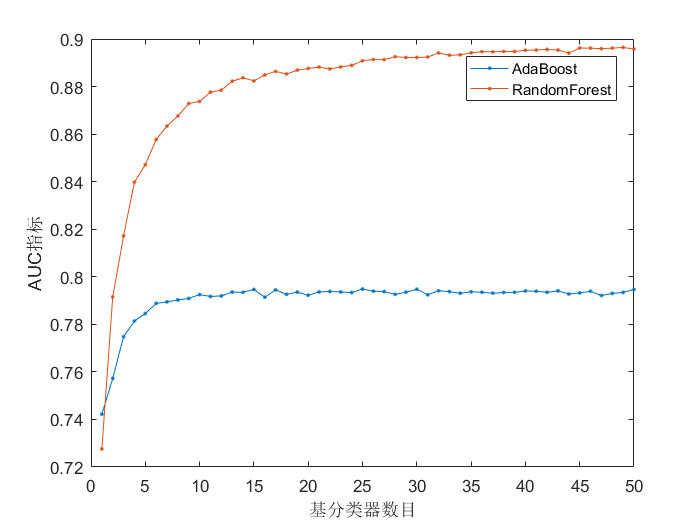
\includegraphics[scale=0.5]{auc.png}
	\caption{AdaBoost和随机森林在不同基分类器数目时的AUC指标}
	\label{fig:label}
\end{figure}
从图中可以看到对于随机森林来说,基分类器在1到15的区间中,AUC上升较快,当基分类器超过40以后,AUC上升就变得十分缓慢。对于AdaBoost来说,基分类器在1到10的区间中,AUC上升较快,超过10之后,AUC的上升十分缓慢。
\item 选取最优的基分类器数目,即选取在交叉验证时AdaBoost和随机森林取得最好AUC的数目,即AdaBoost选取25个基分类器,随机森林选取49个基分类器。在测试集上测试得到的结果如下:
\begin{table}[!ht]
	\centering
	\caption{AdaBoost和随机森林在测试集上的AUC指标}
	\label{my-label}
	\begin{tabular}{|l|l|}
		\hline
	算法	& AUC指标 \\ \hline
	AdaBoost	& 0.8288801089639083 \\ \hline
	随机森林	&  0.8942615694173404\\ \hline
	\end{tabular}
\end{table}\\
\end{enumerate}
以0作为阈值,score大于等于0视为正例,反之视为负例,得到AdaBoost和随机森林其他性能如下:
\begin{table}[!h]
	\centering
	\caption{AdaBoost性能}
	\label{my-label2}
	\begin{tabular}{|l|l|l|l|l|}
		\hline
		& precision & recall & f1-score & support \\ \hline
	负例	& 0.88 & 0.87 & 0.88 & 12435 \\ \hline
	正例	& 0.6 & 0.62 & 0.61 & 3846 \\ \hline
	\end{tabular}
\end{table}
\begin{table}[!h]
	\centering
	\caption{随机森林性能}
	\label{my-label3}
	\begin{tabular}{|l|l|l|l|l|}
		\hline
		& precision & recall & f1-score & support \\ \hline
		负例	& 0.88 & 0.92 & 0.90 & 12435 \\ \hline
		正例	& 0.71 & 0.61 & 0.66 & 3846 \\ \hline
	\end{tabular}
\end{table}
\item 实验结果
本次实验完成了题目的所有要求:包括AdaBoost和随机森林算法的实现,使用交叉验证方法调整参数,在测试集上完成预测并且得到AUC性能指标。\\
实验心得:\\
1.sklearn是非常强大的工具,借助其中的决策树模型可以减轻很多工作量。\\
2.AdaBoost算法虽然不复杂,但是实现过程中会有一些细节性的问题,比如error的计算要加上权重。\\
3.AUC的计算使用score效果会很多。\\
4.使用交叉验证可以方便快捷的进行参数调整。\\
5.将模型实现成class的形式便于coding。
\end{enumerate}
	
\end{document}